\documentclass[10pt,twocolumn,letterpaper]{article}

%%%%%%%%% PAPER TYPE
\usepackage[review]{cvpr}      % review version (line numbers); switch to \usepackage{cvpr} for camera-ready

%% This file contains a number of tweaks that are typically applied to the main document.
%% They are not enabled by default, but can be enabled by uncommenting the relevant lines.

%%
%% Inline annotations; for predefined colors, refer to "dvipsnames" in the xcolor package:
%% https://tinyurl.com/overleaf-colors
%%
\newcommand{\red}[1]{{\color{red}#1}}
\newcommand{\todo}[1]{{\color{red}#1}}
\newcommand{\TODO}[1]{\textbf{\color{red}[TODO: #1]}}
%%
%% disable for camera ready / submission by uncommenting these lines  
%%
% \renewcommand{\TODO}[1]{}
% \renewcommand{\todo}[1]{#1}

%%
%% work harder in optimizing text layout. Typically shrinks text by 1/6 of page, enable
%% it at the very end of the writing process, when you are just above the page limit
%%
% \usepackage{microtype}

%%
%% fine-tune paragraph spacing
%%
% \renewcommand{\paragraph}[1]{\vspace{.5em}\noindent\textbf{#1.}}

%%
%% globally adjusts space between figure and caption
%%
% \setlength{\abovecaptionskip}{.5em}


%%
%% Allows "the use of \paper to refer to the project name"
%% with automatic management of space at the end of the word
%%
% \usepackage{xspace}
% \newcommand{\paper}{ProjectName\xspace}

%%
%% Commonly used math definitions
%%
% \DeclareMathOperator*{\argmin}{arg\,min}
% \DeclareMathOperator*{\argmax}{arg\,max}

%%
%% Tigthen underline
%%
% \usepackage{soul}
% \setuldepth{foobar}

\definecolor{cvprblue}{rgb}{0.21,0.49,0.74}
\usepackage[pagebackref,breaklinks,colorlinks,allcolors=cvprblue]{hyperref}

\def\paperID{****}
\def\confName{CVPR}
\def\confYear{2026}

\newcommand{\method}{\textsc{PPO-CF}}

\title{Reinforcement-Learning-Scheduled Latent Diffusion for Visual Counterfactual\\
Explanations, and What Ground-Truth-Anchored Evaluation Reveals About Them}

\author{Ayoub\\
Independent Research Project\\
}

\begin{document}
\maketitle

\begin{abstract}
Visual counterfactual explanation methods for medical image classifiers
are conventionally scored by Counterfactual Validity (CV): the rate at
which a generated image flips the classifier's decision. We make two
contributions that pull in opposite directions, and argue the second is
the more consequential. First, we present \method{}, a system in which a
PPO agent schedules the sampling procedure of a frozen, LoRA-adapted
latent diffusion generator --- selecting per-step noise strength,
classifier- and preservation-guidance scales, refinement-pass count,
guidance ramp-up point and stopping time --- rather than applying one
hand-tuned schedule to every image, with editing spatially confined to
the lung field by a RePaint-style background lock. Second, we show that
CV, computed as it usually is with the same classifier that guided
generation, is close to uninformative about whether the edit is
class-relevant at all. We introduce two measurements that do not share
that circularity: a Lesion Hit Rate (LHR) anchored to radiologist-drawn
opacity boxes, and a held-out transfer ratio that re-scores
counterfactuals with classifiers that never participated in guidance.
Under these, the picture changes substantially. On the RSNA Pneumonia
Detection Challenge, our committed configuration attains a mean CV of
$0.838$ and a $2.67\times$ LHR lift over the annotation-area null
($p=4.2\times10^{-53}$), yet held-out transfer remains in the adversarial
regime on the most independent validator ($0.046$/$0.186$ against a
$0.15$ threshold). A five-arm study, each arm a policy trained from
scratch and evaluated under an identical protocol, isolates ensemble
guidance as the only tested countermeasure that helps (paired
$d=0.482$) and produces two confirmed negative results: an annealed
sparsity reward fails at its own objective and costs lesion targeting
($d=0.512$), and a Grad-CAM spatial constraint collapses the base task
entirely ($d=1.205$, CV $0.838\to0.017$). We argue that reporting CV
without a ground-truth- or independence-anchored companion metric
systematically overstates progress in this literature.
\end{abstract}

\section{Introduction}

Classifiers deployed on chest radiographs are typically audited with
attribution maps, which indicate \emph{where} evidence is concentrated
but not \emph{what change} would alter the prediction. Visual
counterfactual explanations close this gap: given a query image $x$ with
prediction $f(x)$ and a target class $c$, a generator produces $x_c$ that
(i) is scored at $c$ by the classifier, (ii) remains a realistic
radiograph, and (iii) differs from $x$ only in a minimal, class-relevant
region, preserving anatomy, foreign objects and patient identity.

Two observations motivate this work. The first is a modelling one. A
fixed, hand-tuned guidance schedule is a poor fit across a heterogeneous
test population: some images need only a gentle nudge across the
decision boundary, others require aggressive multi-pass editing, and one
schedule either under-edits the latter or de-realizes the former. We
therefore frame per-step guidance control as a sequential decision
problem and train a PPO agent to schedule it, image-adaptively, against a
reward that trades classification progress against preservation and
realism. Crucially the agent never touches the diffusion weights; it
controls only the sampling procedure around a frozen generator, which
keeps the action space small and the learned policy reusable at
inference time on arbitrary query images.

The second observation is an evaluative one, and in retrospect the more
important. The field's standard success criterion, Counterfactual
Validity, is almost always computed with the same classifier whose
gradients guided generation. It therefore cannot distinguish a genuine
class-relevant edit from an adversarial perturbation tuned to one model.
This is not a hypothetical concern in our setting: our own system reaches
high CV while placing only a minority of its edit mass inside
radiologist-drawn lesion annotations, and while transferring poorly to
classifiers that did not participate in guidance. We consider it a
reporting problem for the subfield rather than a defect specific to our
generator, and we address it with two companion measurements --- one
anchored to human annotation, one to model independence --- that we
recommend alongside CV.

\paragraph{Contributions.}
\begin{enumerate}[leftmargin=*,itemsep=1pt,topsep=2pt]
  \item \method{}: a PPO-scheduled sampling controller over a frozen,
        LoRA-adapted Stable Diffusion generator, with a hard
        segmentation-gated background lock guaranteeing that content
        outside the lung field reconstructs to the autoencoder's
        identity floor (\S\ref{sec:method}).
  \item An evaluation protocol that pairs CV with a ground-truth-anchored
        Lesion Hit Rate and a held-out transfer ratio, together with the
        split-, seeding- and routing-level controls a control-arm
        comparison requires in order to mean anything
        (\S\ref{sec:evalprotocol}).
  \item A five-arm controlled study in which every arm is a policy
        trained from scratch and fully evaluated, yielding one confirmed
        improvement and two confirmed negative results, including the
        largest effect size we measure --- against a mechanism designed
        to help (\S\ref{sec:negresults}).
\end{enumerate}

\section{Related Work}

\paragraph{Counterfactual explanation in medical imaging.} Singla
\emph{et al.}~\cite{singla2022} introduced a GAN-based counterfactual
generator for chest radiographs together with the evaluation protocol
--- Counterfactual Validity, FID, and Foreign-Object Preservation ---
that has become the de facto benchmark, and which we adopt for
comparability. Their FOP metric depends on a Fast R-CNN foreign-object
detector trained on private annotations, which is not reproducible
offline; \S\ref{sec:conventional} describes our model-free substitute.
Subsequent work has largely retained the same classifier-scored notion of
validity~\cite{jeanneret2022dime,jeanneret2023ace,augustin2022dvce}.

\paragraph{Diffusion-based counterfactuals.} Classifier- and
gradient-guided diffusion sampling~\cite{dhariwal2021diffusion,meng2022sdedit,preechakul2022diffae}
has displaced GAN-based approaches for editable generation, owing to more
stable training and higher sample fidelity. We build on a
LoRA-adapted~\cite{hu2021lora} Stable Diffusion v1.5~\cite{rombach2022}
backbone with DDIM sampling~\cite{song2021ddim} rather than training a
diffusion model from scratch on a comparatively small radiograph corpus.

\paragraph{Spatially constrained editing.} RePaint~\cite{repaint} and
Blended Latent Diffusion~\cite{blended} re-noise and re-composite the
unedited region at every denoising step. We adapt this as a hard
background lock: rather than trusting the guidance gradient to keep edits
inside the lung field, the latent outside a dilated, feathered lung mask
is forcibly reset at every step to the original image's forward-diffused
latent.

\paragraph{RL and diffusion.} Most RL work on diffusion fine-tunes the
model \emph{weights} against a reward (e.g.\ DDPO~\cite{black2024ddpo},
reward-weighted fine-tuning). Treating the sampling hyperparameters as an
RL action space around a frozen generator is comparatively unexplored,
and is what we do here.

\section{Method}
\label{sec:method}

\subsection{Problem formulation}
Given a frozen binary classifier $f:\mathcal{X}\to[0,1]$ and a target
class $c\in\{0,1\}$, we seek $x_c$ minimizing
\begin{equation}
\mathcal{L}(x_c) = \underbrace{\mathrm{BCE}(f(x_c),c)}_{\text{classification}}
+ \underbrace{\lambda_{\text{pres}}\,d(x,x_c)}_{\text{preservation}},
\label{eq:objective}
\end{equation}
where $d$ is a masked distance penalizing change inside the segmented
lung field and change to a frozen object-detector embedding (a
foreign-object proxy), and leaving change outside the lung field free ---
subject to the hard lock below, which removes that freedom entirely.

\subsection{Latent generator and background lock}
Images are encoded to a $4\times32\times32$ latent by a frozen SD1.5 VAE.
A lightweight MLP maps $(c, \text{pooled latent})$ to a single
cross-attention conditioning token, replacing SD1.5's text conditioning
with a scalar class signal. Rank-8 LoRA adapters ($\alpha=16$, dropout
$0.05$) are inserted into the UNet's \texttt{to\_q}/\texttt{to\_k}/\texttt{to\_v}/\texttt{to\_out.0}
projections and trained on the standard $\epsilon$-prediction objective
over the training split, adapting the natural-image prior toward
radiography without touching the VAE or the bulk of the UNet.

\textbf{Guided DDIM sampling.} Generation runs a partial, SDEdit-style
forward-then-reverse DDIM trajectory whose length is a \texttt{strength}
fraction of $T_{\text{diff}}=50$ steps, with two gradient terms injected
into the predicted $\hat z_0$ at each step:
\begin{equation}
\Delta z_0 = -w(i)\alpha_{\text{cls}}\nabla_{\hat z_0}\mathcal{L}_{\text{cls}}
- w(i)\alpha_{\text{pres}}\nabla_{\hat z_0}\big(L_1^{\text{seg}} + \eta\,\mathrm{MSE}_{\text{obj}}\big),
\label{eq:guidance}
\end{equation}
gated by a dilated, Gaussian-feathered lung mask $M$ and a linear ramp
$w(i)$ rising from $0$ at a learned fraction of the trajectory, which
avoids the discontinuity of a hard guidance switch.

\textbf{Background lock.} At every step the latent outside $M$ is
overwritten with the original latent forward-noised to the current
timestep (clean at the final step). This is a hard spatial constraint
independent of how the guidance gradient behaves: content outside the
lung field is guaranteed to collapse to the VAE reconstruction floor
rather than being repainted by the free SDEdit process, which is what an
unconstrained high-\texttt{strength} schedule does to the entire thorax.

\begin{table}[t]
\centering
\small
\caption{Action space. All nine dimensions are emitted per refinement
step, so the schedule is adaptive both across images and within an
episode.}
\label{tab:actionspace}
\begin{tabular}{@{}lll@{}}
\toprule
& \textbf{Controls} & \textbf{Range} \\
\midrule
$a_0$ & DDIM strength & $[0.20,0.70]$ \\
$a_1$ & classifier-guidance scale & $[0.5,3.0]$ \\
$a_2$ & preservation-guidance scale & $[0.3,1.5]$ \\
$a_3$ & stop signal $\tau_t$ & $[0,1]$ \\
$a_4,a_5$ & extra refinement pass (Bernoulli) & $\{0,1\}$ \\
$a_6$ & per-pass strength boost & $[0.85,1.15]$ \\
$a_7$ & guidance bias (cls vs.\ pres) & $[0.70,1.30]$ \\
$a_8$ & guidance ramp-up start fraction & $[0.1,0.5]$ \\
\bottomrule
\end{tabular}
\end{table}

\subsection{PPO-scheduled sampling}
Rather than fixing \texttt{strength}, guidance scales and pass count, a
PPO agent~\cite{schulman2017ppo} emits a 9-dimensional continuous action
at each of up to $T=25$ refinement steps, mapped through sigmoid
transforms to the controls in Table~\ref{tab:actionspace}.

The observation concatenates the flattened original and current latents,
the normalized step index, the current $|f(x_t)-c|$, the target $c$, and
the flattened lung mask. Episodes terminate when $|f(x_t)-c|<\varepsilon_{\text{stop}}=0.08$
or the budget is exhausted.

\textbf{Reward.} The per-step reward combines progress toward the
target, a fidelity penalty against the original, a mask-weighted
preservation penalty plus a foreign-object-embedding KL term, a per-step
budget cost, and terminal bonuses for reaching validity and for stopping
once valid, weighted as in the supplementary configuration.

\textbf{Architecture.} A shared $512\to256$ MLP trunk feeds a Gaussian
policy head with per-dimension learnable log-std, a value head, and
three auxiliary heads (feasibility, progress, stop) trained alongside the
clipped PPO objective with GAE ($\gamma=0.99$, $\lambda_{\text{GAE}}=0.95$).

\subsection{Directional policies}
The environment is built around a fixed target, so one policy is trained
for n$\to$p ($c=1$) and another for p$\to$n ($c=0$), sharing the
generator but specializing their schedules. This follows an asymmetry we
observe throughout: synthesizing a plausible, spatially coherent opacity
pattern in a clean lung field is a harder and more under-constrained
generative problem than removing one, which is closer to an inpainting
operation the pretrained prior already performs well.

\section{Evaluation Protocol}
\label{sec:evalprotocol}

\subsection{Conventional metrics}
\label{sec:conventional}
Following~\cite{singla2022}, the evaluation set is split by classifier
confidence into $X_n=\{x:f(x)<0.2\}$ and $X_p=\{x:f(x)>0.8\}$, up to
$n_{\text{eval}}=200$ each, and each directional policy generates from
the corresponding group with its deterministic (mean) action.

\textbf{Counterfactual Validity.} We tighten the original,
direction-agnostic definition to
\begin{equation}
\mathrm{CV} = \Pr\big[\,|f(x_c)-f(x)|>\tau \wedge \mathrm{sign}(f(x_c)-0.5)=c\,\big],
\label{eq:cv}
\end{equation}
with $\tau=0.8$, so that an image moving the wrong way by a large margin
is no longer silently credited.

\textbf{FID.} Computed on penultimate-layer features of a
TorchXRayVision DenseNet-121~\cite{cohen2020xrv} rather than ImageNet
Inception-v3, since it is trained on the same source distribution and
yields a feature space sensitive to pneumonia-relevant structure rather
than generic natural-image texture. Covariances are regularized
($\epsilon=10^{-6}$) before the matrix square root, since the sample
count is below the feature dimensionality.

\textbf{Identity Preservation (IP).} As a dependency-free substitute for
FOP we report MS-SSIM (global anatomical identity across scales) and
HF-corr, the Pearson correlation of high-pass-filtered images --- a
direct proxy for whether thin, high-contrast structures such as tubes,
leads and pacemakers survive editing, since those are exactly the
spatial frequencies a Gaussian high-pass isolates.

\subsection{Ground-truth-anchored Lesion Hit Rate}
CV, FID and IP share a blind spot: none of them can tell whether the
edit landed on the pathology. RSNA ships $9{,}555$ radiologist-drawn
opacity boxes, which we retain. LHR measures the fraction of an edit's
absolute-difference mass falling inside the annotation, against the
box's own area as the null; \emph{lift} (hit rate over null), not raw hit
rate, is therefore the informative quantity. LHR is defined only for
p$\to$n, since n$\to$p sources are classifier-negative and carry no
annotation.

We calibrate the metric before use on synthetic edits with known ground
truth: a uniform wash scores lift $1.00$ ($p=0.59$, chance, as it
should), an on-lesion edit scores $12.4$ ($p=3\times10^{-49}$), an
off-lesion edit scores $0$.

\subsection{Held-out transfer}
Because CV is computed with the guidance classifier, it cannot separate
a class-relevant edit from an adversarial perturbation. We therefore
re-score every counterfactual with classifiers that never participated
in guidance --- \texttt{nih}, \texttt{pc}, \texttt{mimic\_ch} --- and
report the ratio of their score shift to the guidance model's own. A
ratio below $0.15$ we treat as the adversarial regime. The denominator
is read from each shard's own recorded configuration stamp rather than
from the live configuration, so that a validator which never
participated in guidance cannot dilute a denominator it never optimized.

\subsection{Controls the comparison requires}
A control-arm comparison is only as trustworthy as the plumbing beneath
it, and three preconditions we had assumed did not hold. (i) A single
dataset object was shared by LoRA fine-tuning, the PPO pool and the
metrics scan, so evaluation images had been seen during fine-tuning; we
replace this with one deterministic, persisted, \emph{patient-level}
split shared by every stage, computed once because generation runs as
independent array processes that cannot recompute an RNG-based split
consistently. (ii) Training was unseeded --- two identical submissions
produced two different policies, survivable for a headline number but
not for a comparison in which arms must differ by treatment alone.
(iii) The control arms had never been exercised: wiring them up surfaced
a routing bug under which every reduce silently fell back to the trained
arm's shards, which would have made ``the policy contributes nothing''
an artefact of a missing flag, and a shared output directory under which
each arm overwrote the previous one's metrics. A CPU-only invariant
suite pins the LHR calibration, split disjointness and three further
properties whose silent failure would yield a plausible-looking wrong
number rather than a crash.

We report these because each was, at the time it was found, invisible in
the outputs: all three would have produced a well-formed table.

\section{Experiments}
\label{sec:experiments}

\subsection{Setup}
We use the RSNA Pneumonia Detection Challenge dataset~\cite{rsna} (DICOM,
min--max normalized, resized to $256\times256$, binary label collapsed
from bounding-box annotations). The guidance classifier is a
TorchXRayVision DenseNet-121 (\texttt{densenet121-res224-rsna});
segmentation uses TorchXRayVision PSPNet for lung and heart channels; a
YOLOv8n feature extractor supplies the foreign-object embedding. Each
policy is trained for 800 episodes per direction; the two directions
take 8h40m and 11h00m respectively on a single node.

\subsection{Main results}
Table~\ref{tab:main} reports the committed configuration (2-model
guidance ensemble, no Grad-CAM mask, no sparsity reward).

\begin{table}[t]
\centering
\small
\caption{Committed configuration, $n=200$ per group. LHR is defined only
for p$\to$n.}
\label{tab:main}
\begin{tabular}{@{}llrr@{}}
\toprule
\textbf{Metric} & & \textbf{n$\to$p} & \textbf{p$\to$n} \\
\midrule
CV & fraction valid, $\tau{=}0.8$ & 0.960 & 0.715 \\
   & \emph{mean} & \multicolumn{2}{c}{0.838} \\
LHR lift & vs.\ annotation-area null & --- & 2.673 \\
   & \multicolumn{3}{l}{\footnotesize $t{=}24.19$, $p{=}4.2\times10^{-53}$, $n{=}148$} \\
Transfer & mean over 3 validators & 0.282 & 0.293 \\
EditConc. & top-5\% mass (uniform${=}0.05$) & 0.253 & 0.318 \\
   & fraction of pixels changed & 0.650 & 0.633 \\
FID & vs.\ real target class & 22.21 & 4.95 \\
IP & MS-SSIM & 0.923 & 0.870 \\
IP & HF-corr & 0.948 & 0.914 \\
\bottomrule
\end{tabular}
\end{table}

\begin{table}[t]
\centering
\small
\caption{Held-out transfer ratio, single- vs.\ ensemble-guided trained
policies, $n=200$ per group. Values below $0.15$ are in the adversarial
regime.}
\label{tab:transfer}
\resizebox{\linewidth}{!}{%
\begin{tabular}{@{}lrrrrrr@{}}
\toprule
& \multicolumn{2}{c}{nih} & \multicolumn{2}{c}{pc} & \multicolumn{2}{c}{mimic\_ch} \\
Policy & n$\to$p & p$\to$n & n$\to$p & p$\to$n & n$\to$p & p$\to$n \\
\midrule
Single-classifier & 0.080 & 0.100 & 0.414 & 0.224 & 0.197 & 0.112 \\
2-model ensemble & 0.046 & 0.186 & 0.462 & 0.308 & 0.337 & 0.384 \\
\bottomrule
\end{tabular}%
}
\end{table}

Three things are worth reading together. The policy succeeds at the base
task in the easier direction and less so in the harder one. It
concentrates edit mass on radiologist-annotated lesions far above chance
--- a $2.67\times$ lift is not a marginal effect. And yet it changes
roughly $65\%$ of pixels and places only about a quarter of its
difference mass in the top $5\%$ of the edit map, against a $0.05$
uniform baseline and a $\sim\!0.5$ threshold we would associate with a
focal, lesion-shaped edit. The edits are class-informative and diffuse
at the same time.

\subsection{CV overstates what the edits achieve}
\label{sec:overstates}
Table~\ref{tab:transfer} makes the case directly. Moving from
single-classifier to 2-model ensemble guidance \emph{lowers} mean CV
from $0.965$ to $0.838$ while \emph{raising} LHR lift from $2.293$ to
$2.673$ and raising mean held-out transfer on both directions. A harder
joint criterion is not a weaker policy, and the metric that fell is the
one that shares a classifier with the generator.

A single-run point estimate cannot resolve the apparent \texttt{nih}
regression, so we bootstrap it ($10{,}000$ percentile resamples of the
$n=200$ groups, numerator and denominator resampled jointly to preserve
within-image pairing). For n$\to$p, $[0.048,0.114]$ vs.\ $[0.007,0.084]$:
the intervals overlap substantially and the apparent worsening is not
distinguishable from noise --- but both sit entirely below $0.15$, so
what \emph{is} established is that n$\to$p stays confidently adversarial
under either policy. For p$\to$n, $[0.076,0.126]$ vs.\ $[0.155,0.216]$ do
not overlap, so that improvement is real. We report each policy's
interval separately rather than a difference-of-ratios bootstrap, because
the classifier that sorts images into $X_n$/$X_p$ changed between runs
and the two groups share only $\approx70\%$ (n$\to$p) and $\approx24\%$
(p$\to$n) of their members; a paired resample would synthesize a pairing
that is not there.

This is the paper's central empirical claim. A system reporting CV
$0.965$ and, on the most independent validator, a transfer ratio of
$0.08$ is not producing explanations of the pathology; it is producing
perturbations that a second model largely does not see. Nothing in the
conventional metric suite surfaces that.

\subsection{Five trained arms}
\label{sec:fivearms}
Every arm in Table~\ref{tab:fivearm} is a policy trained from scratch
for 800 episodes per direction and evaluated end-to-end under the
identical protocol --- not a cheaper no-policy sweep or an offline proxy.
Verdicts are paired significance tests on the images two arms share,
never differences of group means.

\begin{table}[t]
\centering
\small
\caption{Five trained-and-evaluated arms. Bold marks the arm no other arm
beats under a paired test or bootstrap CI, not the best point estimate.
$^{*}$scored on the reduced leak-free validator set \{nih,pc\}; not
comparable to the other rows' 3-validator mean.}
\label{tab:fivearm}
\begin{tabular}{@{}lrrl@{}}
\toprule
\textbf{Arm} & \textbf{LHR} & \textbf{Transfer} & \textbf{vs.\ default} \\
\midrule
Single-classifier & 2.293 & 0.230/0.146 & worse ($d{=}0.482$) \\
\textbf{2-ens (default)} & \textbf{2.673} & \textbf{0.282/0.293} & --- \\
3-model ensemble & 2.492 & 0.350/0.276$^{*}$ & unresolved ($n{=}12$) \\
Sparsity reward & 2.398 & 0.311/0.212 & worse ($d{=}0.512$) \\
Grad-CAM constraint & 1.636 & 0.161/0.103 & much worse ($d{=}1.205$) \\
\bottomrule
\end{tabular}
\end{table}

\begin{figure}[t]
\centering
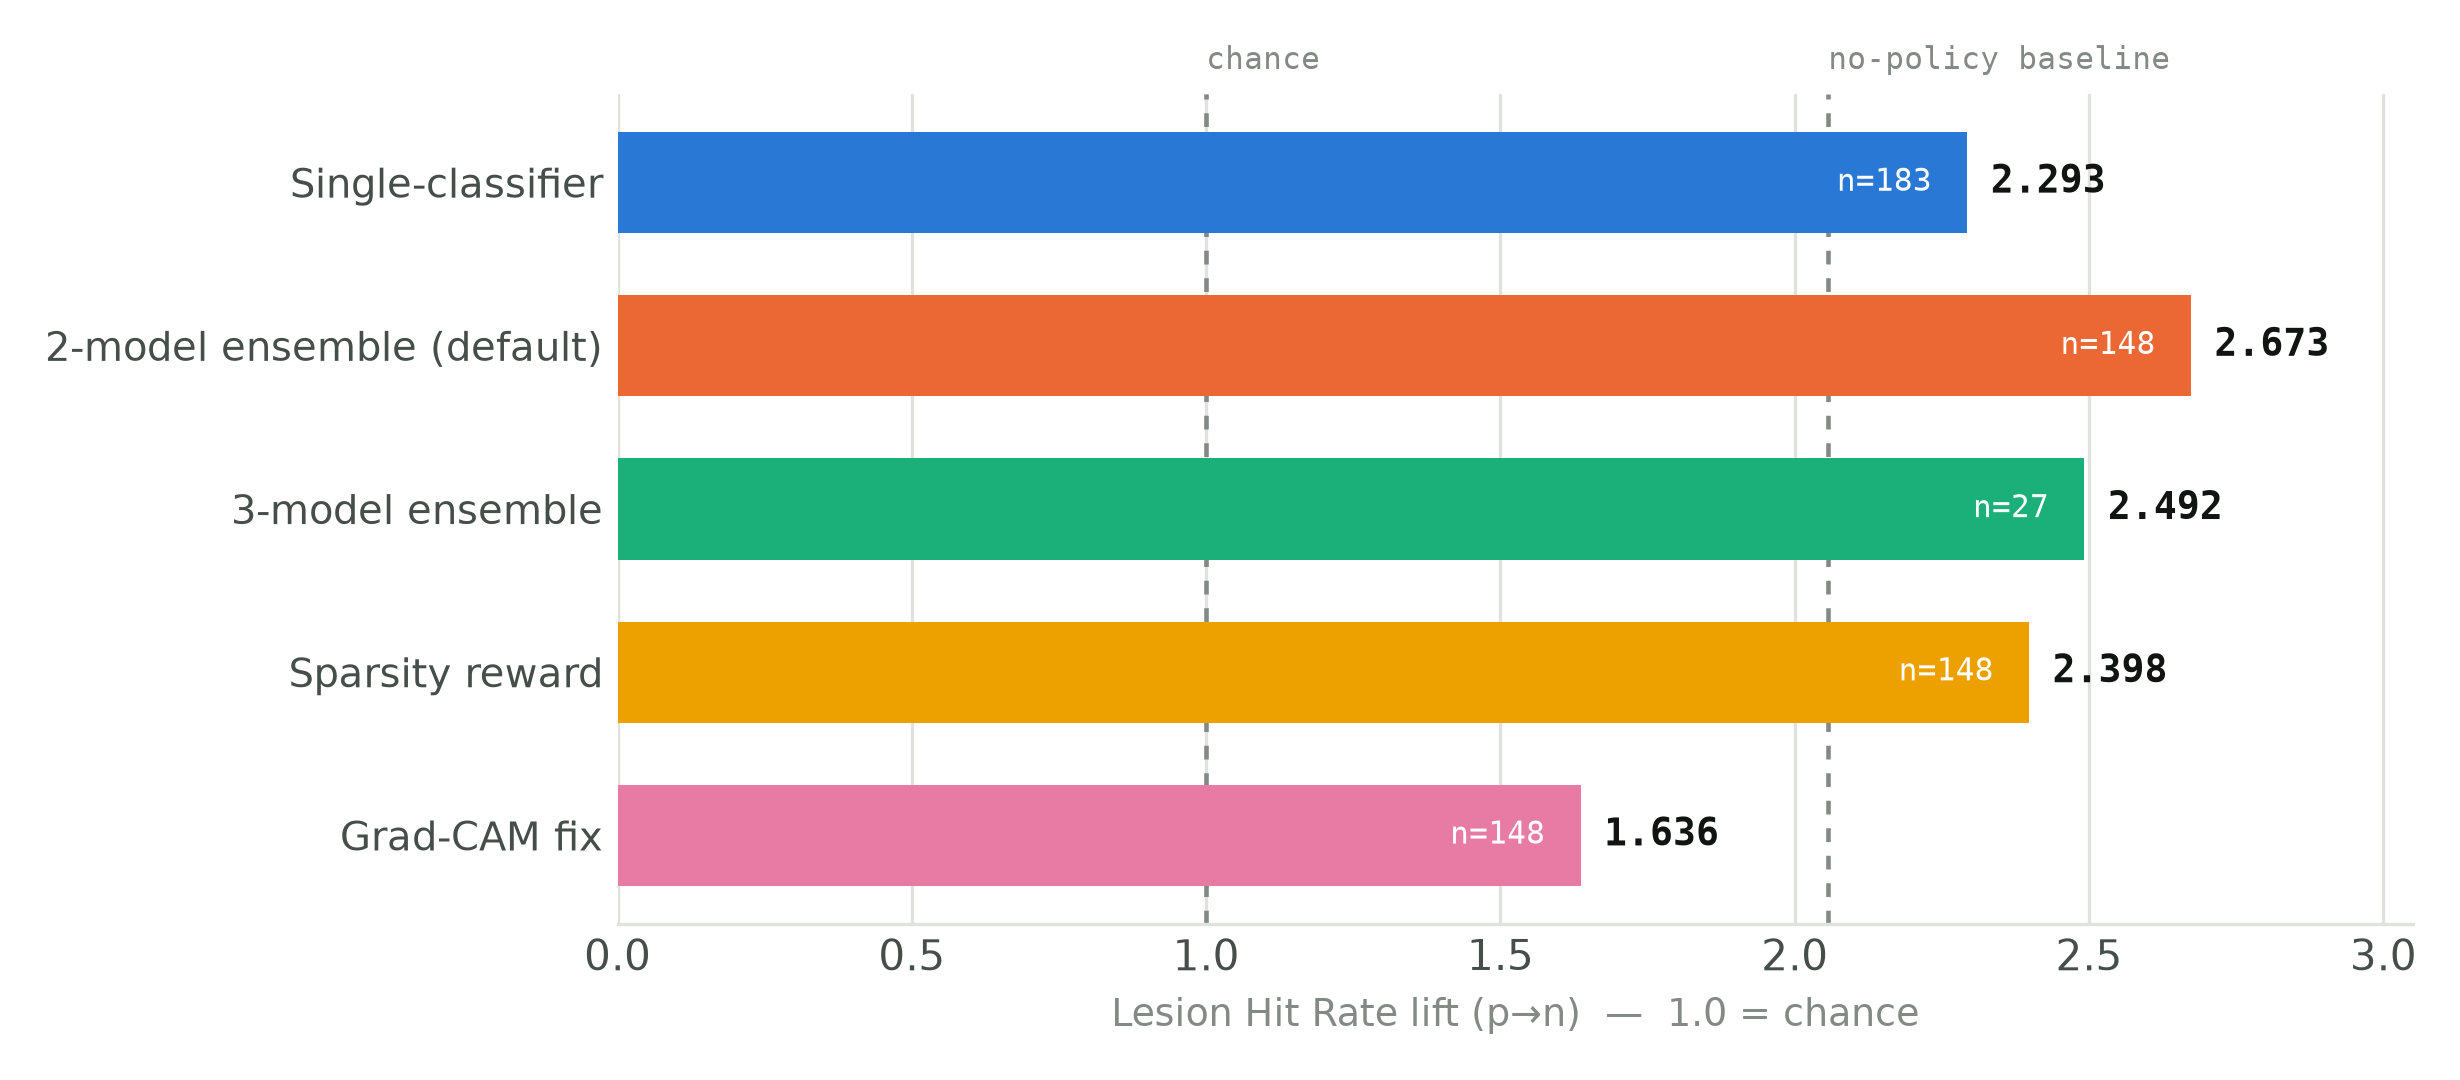
\includegraphics[width=\linewidth]{figures/chart_lhr_lift.png}
\caption{LHR lift (p$\to$n) across all five trained arms. Dashed lines
mark chance ($1.0$) and the no-policy label-protocol baseline ($2.057$).}
\label{fig:lhr}
\end{figure}

\textbf{Ensemble guidance helps, and the effect replicates.} Paired
per-image LHR-lift deltas across three independent seeds are $+0.0694$
($d=0.221$), $+0.0693$ ($d=0.223$) and $+0.0575$ ($d=0.151$), all with
$95\%$ CIs excluding zero. The single-classifier$\to$2-model step is
confirmed on the 76 shared annotated images ($d=0.482$,
$p=7.1\times10^{-5}$). Growing the ensemble to three members improves
\texttt{pc} n$\to$p transfer from $0.462$ to $0.623$ with non-overlapping
CIs, moves \texttt{nih} in the right direction on both counts without
separating from noise, and does not resolve on LHR --- only 12 annotated
images are shared between the two arms, giving a paired CI of
$[-0.298,+0.482]$. Ensemble size buys resistance to fooling an
independent classifier, not sharper lesion targeting; the two properties
dissociate.

\textbf{The trained policy beats a random one, but barely.} Against the
random-action arm on the same 183 images: paired lift difference
$+0.090$ ($95\%$ CI $[+0.021,+0.160]$), $t=2.551$, $p=0.0116$, Wilcoxon
$p=0.0147$, $d=0.189$, trained better on 105/183. Real, small, and
considerably smaller than either negative result below.

\subsection{Two negative results}
\label{sec:negresults}

\textbf{An annealed sparsity reward fails at its own objective.} Edit
concentration has stayed in the $0.25$--$0.32$ band in every arm we
measure. The sparsity term was built to address this and had been
disabled throughout, leaving its annealing ramp inert. Enabled and
isolated against the default, with $\lambda_{\text{sparsity}}$ confirmed
ramping to its target, concentration moved by less than $0.02$ and the
fraction of pixels changed by less than $0.01$. Meanwhile a paired test
on the 148 shared annotated images gives a lift gap of $+0.275$
favouring the arm \emph{without} it ($95\%$ CI $[+0.188,+0.363]$,
$t=6.229$, $p=4.7\times10^{-9}$, $d=0.512$), and p$\to$n transfer falls
from $0.293$ to $0.212$ with non-overlapping CIs on two of three
validators. Without a working spatial mask the term degrades to plain
unweighted $L_1$, which discourages edit mass uniformly rather than
off-target mass specifically --- a plausible account of why it competes
with precise editing while failing at its own goal.

\textbf{A Grad-CAM spatial constraint collapses the base task.}
Constraining edits to a Grad-CAM~\cite{selvaraju2017gradcam} region
lowered LHR lift rather than raising it, so we diagnosed it directly.
Scoring 263 member-image observations under the exact ensemble Grad-CAM
path used during training contradicted the explanation on record: it is
\texttt{chex}, not \texttt{rsna}, that degenerates (66/263, $25.1\%$ vs.\
1/263), and it does so concentrated at \emph{low} predicted probability
rather than near $0.5$ --- consistent with output saturation zeroing the
gradient. When \texttt{chex} degenerates the averaged mask falls back
toward the least-constrained member alone, and CAM--lesion overlap falls
with it ($2.052$, $n=127$ on clean episodes vs.\ $1.347$, $n=23$ on
partially degenerate ones). The remedy on record --- a finer target layer
--- does eliminate the degeneracy ($0\%$/$0.4\%$) but drops baseline
CAM--lesion lift to $1.196$, barely above chance.

Trained for real under that remedy, the result is unambiguous: CV
collapses from $0.838$ to $0.017$, the paired LHR gap is $+1.037$
favouring the unconstrained arm ($95\%$ CI $[+0.900,+1.178]$,
$t=14.660$, $p=1.5\times10^{-30}$, $d=1.205$, better on 141/148 images),
and transfer falls across all three validators. This is the largest
paired effect size we measure anywhere, and it is against a mechanism
introduced specifically to help. Constraining the action space to a
finer, less confident CAM region does not trade a degeneracy problem for
a localisation problem; it makes the base task substantially harder and
every dependent metric degrades with it.

\subsection{Clinical proxy metrics}
\label{sec:clinical}
We additionally report two clinically motivated proxies under the
committed configuration: the Cardio-Thoracic Ratio (CTR), the ratio of
heart-mask to lung-mask horizontal span, and a costophrenic-recess score
(SCP) approximating pleural blunting, each tested with a paired
$t$-test on the within-image real-to-counterfactual delta.

CTR shifts by $+0.0076$ ($t=2.246$, $p=0.026$) in n$\to$p and by
$+0.0080$ ($t=1.010$, $p=0.314$) in p$\to$n: a small, only
one-directionally significant shift, with an absolute magnitude
($<0.01$) far below the metric's clinical resolution (its diagnostic
threshold sits at $0.5$). This is consistent with the intended behaviour
of the background lock, since the cardiac silhouette lies largely
outside the lung mask that gates editing --- we do not read it as a
confident, clinically directional CTR effect, only as a shift too small
to act on either way. SCP's own computation flags itself as degenerate
under this configuration (relative spread $0.19\%$ across the four
comparison groups), so its delta and $t$-test are withheld rather than
reported on what is, numerically, a near-constant signal; built on a
COCO-pretrained detector's feature norm rather than a dedicated recess
detector, we do not consider it informative in its current form. Neither
clinical proxy currently supports a directional claim about pleural or
cardiac status; both should be read as evidence the edit is not
clinically inert at best, not as measurements of a specific clinical
change.

\subsection{Comparison to prior methods}
\label{sec:comparison}
No Vanilla CycleGAN or GANterfactual training or evaluation artifact
exists in our own pipeline, so Table~\ref{tab:baseline} reports both as
literature-reported reference values rather than same-protocol
measurements: they were not re-run under \S\ref{sec:evalprotocol}'s
split, seeding, or evaluation procedure, and should be read as indicative
context, not a controlled comparison. Relative to GANterfactual's
reported FID, ours is better by $1.13\times$ (n$\to$p, $22.21$ vs.\
$25.0$) and $4.04\times$ (p$\to$n, $4.95$ vs.\ $20.0$); our mean CV
($0.838$) is lower than GANterfactual's reported $0.9725$, which is
expected under our protocol rather than a shortfall, since the committed
configuration explicitly trades CV for the classifier-independent
validity documented in \S\ref{sec:overstates} rather than optimizing CV
in isolation.

\begin{table}[t]
\centering
\small
\caption{Literature-reported reference values (Vanilla CycleGAN,
GANterfactual~\cite{singla2022}), not re-run under our protocol, vs.\ our
committed configuration (measured, Table~\ref{tab:main}).}
\label{tab:baseline}
\begin{tabular}{@{}lrrr@{}}
\toprule
\textbf{Method} & \textbf{CV} & \textbf{FID n$\to$p} & \textbf{FID p$\to$n} \\
\midrule
CycleGAN (lit.) & 0.385 & 55.0 & 45.0 \\
GANterfactual (lit.) & 0.973 & 25.0 & 20.0 \\
\textbf{\method{} (ours, measured)} & 0.838 & \textbf{22.21} & \textbf{4.95} \\
\bottomrule
\end{tabular}
\end{table}

\subsection{Qualitative examples}
\label{sec:qualitative}
Figure~\ref{fig:qualitative} shows representative counterfactuals from
the committed configuration in both edit directions, generated with each
policy's deterministic (mean) action. In both examples the classifier
score fully saturates toward the target, well beyond the CV validity
margin, and gross anatomical layout --- rib cage, mediastinal silhouette,
external hardware --- is visibly retained outside the edited lung region:
the qualitative signature of the background lock holding as intended.
The p$\to$n edit is visibly more concentrated than the n$\to$p one,
consistent with \S\ref{sec:method}'s directional asymmetry and with
p$\to$n's lower FID (Table~\ref{tab:main}), though both remain diffuse
relative to a purely lesion-shaped edit (\S\ref{sec:fivearms}).

\begin{figure}[t]
\centering
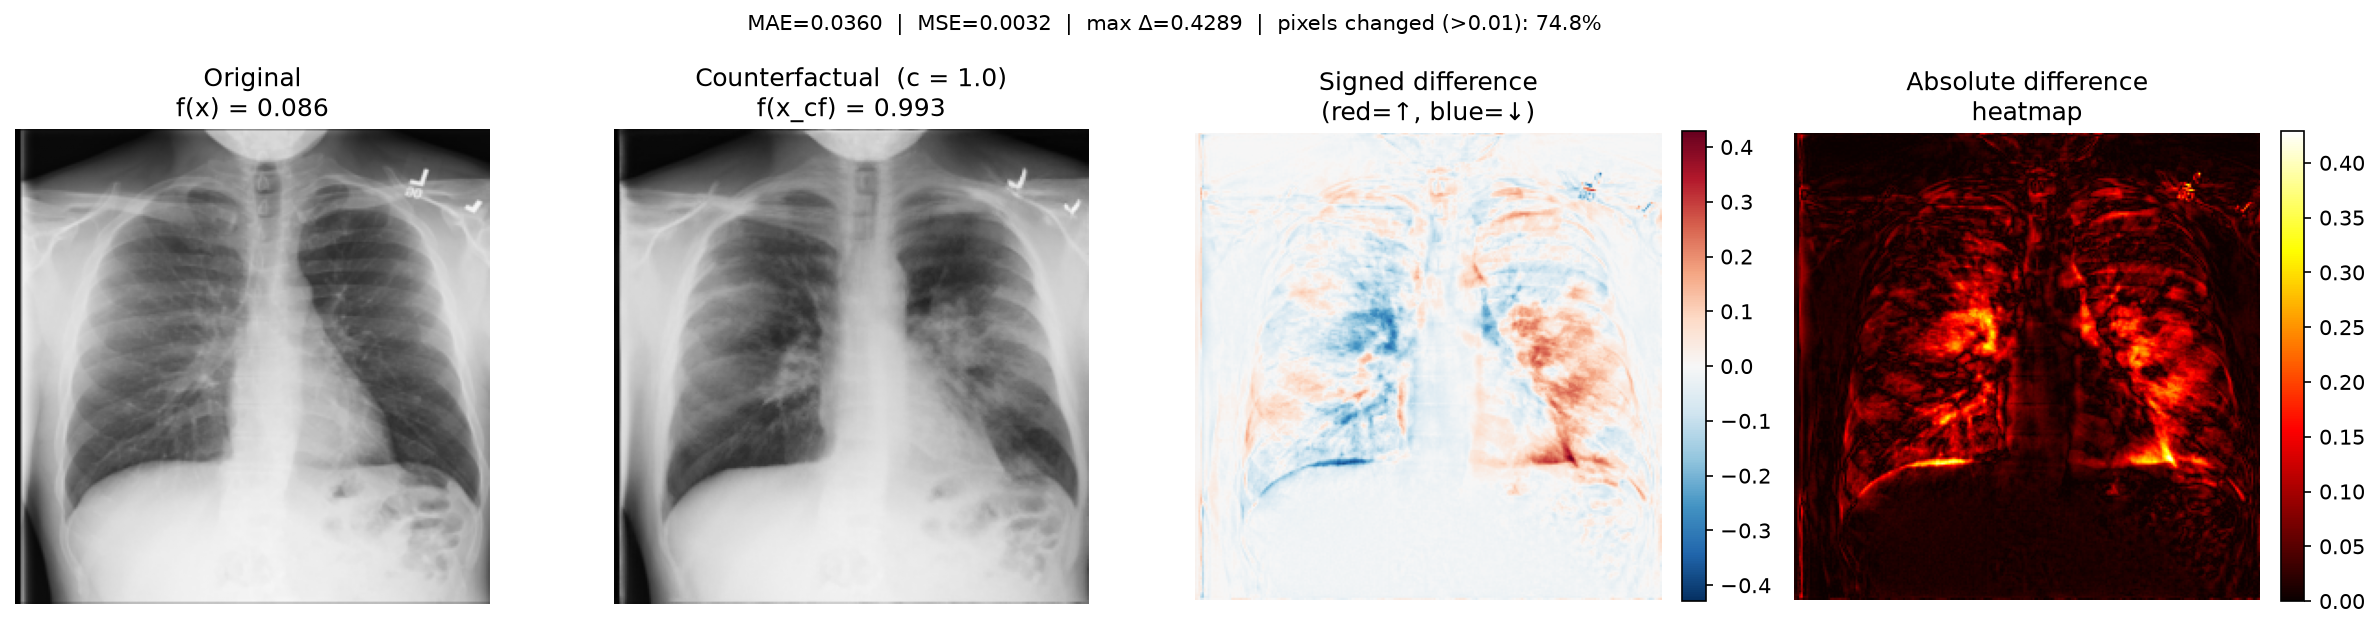
\includegraphics[width=\linewidth]{figures/counterfactual_diff_n_to_p.png}
\caption{n$\to$p. Original, counterfactual, signed difference, absolute
difference. Change is concentrated over the lung fields where an opacity
is synthesized, with anatomy outside the lung mask retained.}
\label{fig:qualitative}
\end{figure}

\begin{figure}[t]
\centering
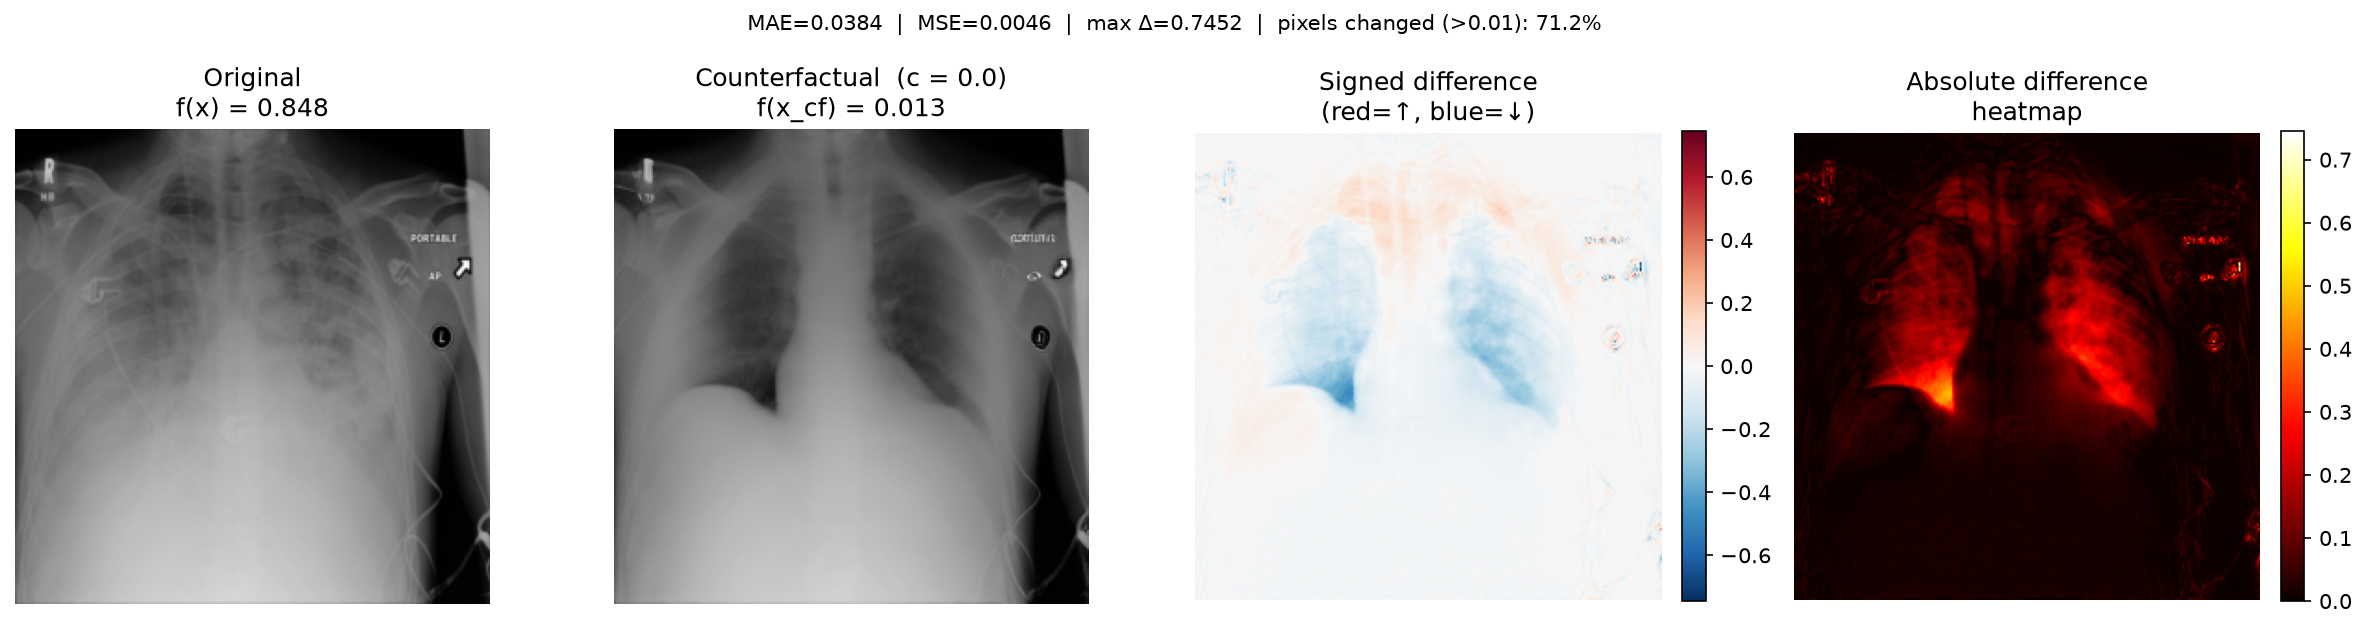
\includegraphics[width=\linewidth]{figures/counterfactual_diff_p_to_n.png}
\caption{p$\to$n. Original, counterfactual, signed difference, absolute
difference. Change concentrates bilaterally over both lung fields,
consistent with opacity removal, while gross anatomy and external
hardware outside the lung mask are retained --- the qualitative signature
of the background lock holding.}
\label{fig:qualitative-pn}
\end{figure}

\section{Limitations}
\label{sec:limitations}

\begin{itemize}[leftmargin=*,itemsep=1pt,topsep=2pt]
  \item \textbf{Edits remain diffuse.} No arm we trained moved edit
        concentration meaningfully; every one sits in the same
        $0.21$--$0.32$ band regardless of what changed underneath it.
        Whether diffuseness is fixable at all within a gradient-guidance
        approach is open.
  \item \textbf{n$\to$p stays adversarial.} On the most independent
        validator, both policies sit confidently below the $0.15$
        threshold. We can show ensemble guidance is a partial
        countermeasure; we cannot show the gap closes.
  \item \textbf{FOP is not computable offline}, so IP measures a related
        but not identical property, and SCP is a coarse proxy rather
        than a trained detector --- and is, in the committed
        configuration, degenerate rather than merely coarse
        (\S\ref{sec:clinical}).
  \item \textbf{Sample size limits several verdicts}, notably the
        3-model ensemble's LHR comparison ($n=12$ shared annotated
        images) and FID, whose variance at $n\sim200$ in a 1024-d feature
        space is high.
  \item \textbf{Two independent policies} rather than one
        target-conditioned policy; the harder direction cannot borrow
        capacity from the easier one.
\end{itemize}

\section{Conclusion}

We presented a PPO-scheduled, LoRA-adapted latent diffusion pipeline for
visual counterfactual explanation on chest radiographs, with a hard
background lock confining edits to the lung field, and evaluated it
under a protocol that pairs the field's conventional classifier-scored
validity with a lesion-annotation-anchored hit rate and a held-out
transfer ratio. The system attains a $2.67\times$ lesion-targeting lift
over chance and improves transfer under ensemble guidance, replicated
across seeds. It also shows, on its own outputs, that high CV coexists
with diffuse edits and adversarial-regime transfer on the most
independent validator --- and that the configuration change which most
improves the anchored metrics is the one that \emph{lowers} CV. Two
mechanisms designed to concentrate edits were trained and measured rather
than assumed, and both are confirmed harmful, one by the largest effect
size in the study. We take the broader implication to be methodological:
CV computed with the guidance classifier should not be reported as a
standalone success criterion, and an anchored companion metric --- to
human annotation, to model independence, or both --- costs little and
changes the conclusion.

{
    \small
    \bibliographystyle{ieeenat_fullname}
    \bibliography{paper}
}

\end{document}
